% Mean + change and mean + self-similarity (Section 4.5) worked on a toy example: 3 frames x 4 features.
% Made-up numbers, already standardized. Checked with a script (20 Nov):
%   mean = (0.2, -0.1, 0.4, 0.4); |x2-x1| = (0.3, 0.3, 0.3, 0.0); |x3-x2| = (1.8, 1.8, 0.9, 0.3);
%   change = (1.05, 1.05, 0.60, 0.15); cos(x1,x2) = 0.934, cos(x1,x3) = -0.723, cos(x2,x3) = -0.732.
% Colors follow frame-combinations.tex: blue = mean of the frames, purple = temporal information added to it.
\documentclass[12pt,border=10pt]{standalone}
% Shared style for the slide figures: sans-serif text (Helvetica, close to the Arial of the charts),
% the same colors as charts.py, and the manuscript's table tools.
\usepackage[T1]{fontenc}
\usepackage[scaled]{helvet}
\renewcommand{\familydefault}{\sfdefault}
\usepackage{amsmath,amssymb}
\usepackage{sansmath}
\usepackage{xcolor}
\usepackage{booktabs,array}
\newcolumntype{L}[1]{>{\raggedright\arraybackslash}p{#1}}
\usepackage{tikz}
\usetikzlibrary{arrows.meta,positioning,calc}

\definecolor{ink}{HTML}{0B0B0B}
\definecolor{inktwo}{HTML}{52514E}
\definecolor{muted}{HTML}{898781}
\definecolor{gridc}{HTML}{E1E0D9}
\definecolor{basec}{HTML}{C3C2B7}
% one color per selection rule, in the fixed categorical order of the charts
\definecolor{cp}{HTML}{2A78D6}     % k-Changepoint (content)
\definecolor{sme}{HTML}{EB6834}    % SME (position)
\definecolor{posc}{HTML}{1BAF7A}    % positional (position)
\definecolor{rnd}{HTML}{EDA100}    % random (chance)
\definecolor{bocpd}{HTML}{E87BA4}  % k-BOCPD (content), categorical slot 5
\definecolor{temporal}{HTML}{6250D6}  % temporal information added to the mean (frame combinations figure)

\newcommand{\chip}[1]{\tikz[baseline=0.1ex]\fill[#1, rounded corners=1pt] (0,0) rectangle (0.32cm,0.32cm);}
\AtBeginDocument{\sansmath\color{ink}}
\hyphenpenalty=10000 \exhyphenpenalty=10000   % no hyphenated words on slides

\newcommand{\cells}[5]{% #1 x start, #2 y, #3 cell width, #4 fill, #5 values
   \foreach \v [count=\i from 0] in {#5} {
      \node[draw=white, line width=1.2pt, fill=#4, minimum width=#3 cm, minimum height=0.6cm, inner sep=0pt,
            font=\small, anchor=west] at (#1+\i*#3, #2) {\v};
   }}
\newcommand{\rowlabel}[3]{\node[anchor=east, font=\small, text=inktwo] at (#1, #2) {#3};}
\begin{document}
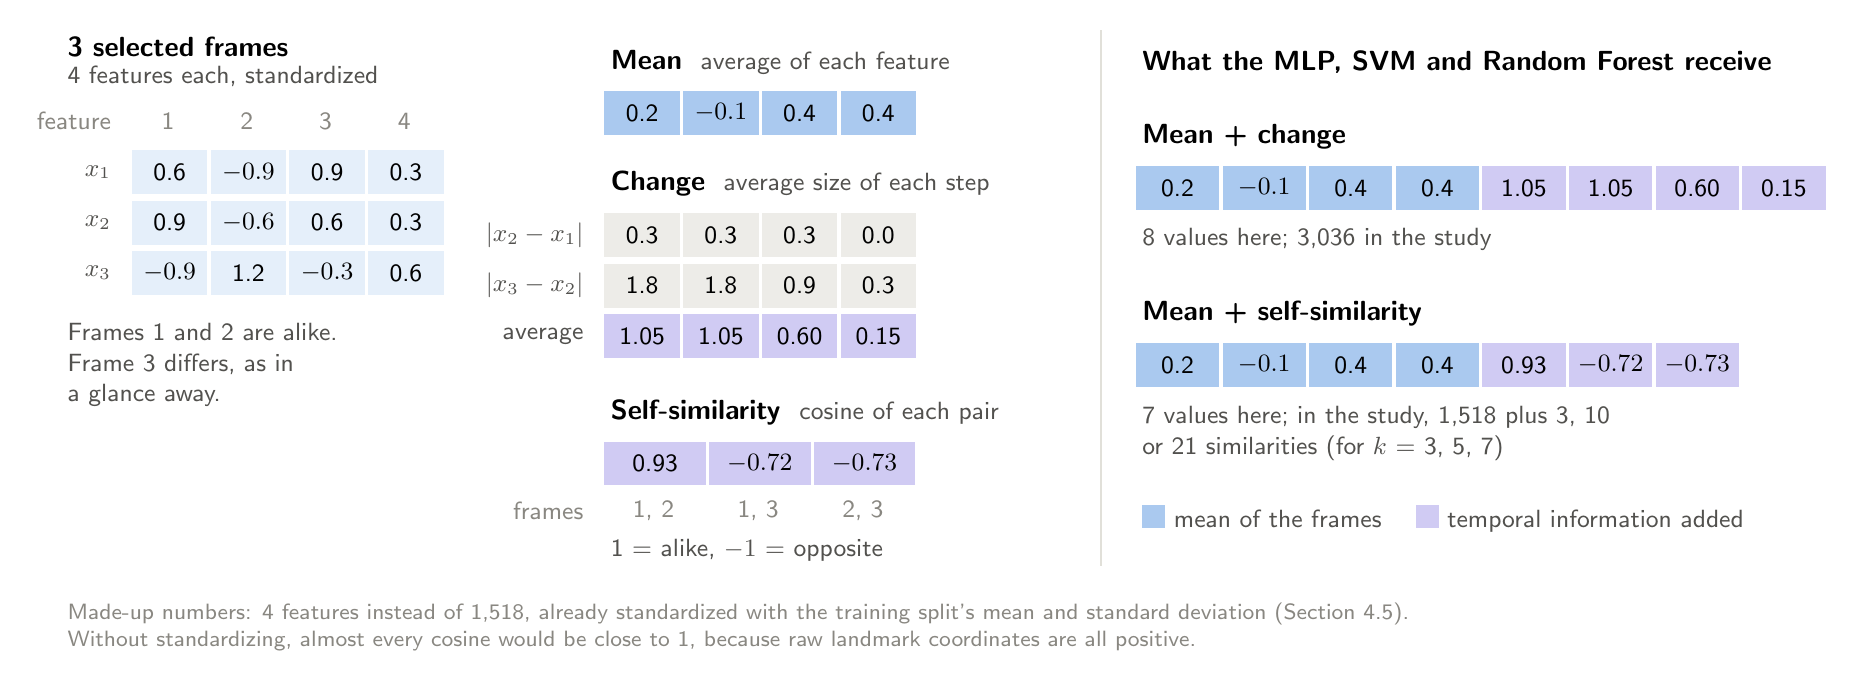
\begin{tikzpicture}
   % ---------- column 1: the selected frames
   \node[anchor=west, align=left] at (-0.9, 1.2) {\textbf{3 selected frames}\\[-2pt]\small\textcolor{inktwo}{4 features each, standardized}};
   \rowlabel{-0.1}{0.45}{\textcolor{muted}{feature}}
   \foreach \f [count=\i from 0] in {1,2,3,4} \node[font=\small, text=muted] at (0.5+\i*1.0, 0.45) {\f};
   \rowlabel{-0.1}{-0.2}{$x_1$}  \cells{0}{-0.2}{1.0}{cp!12}{0.6, $-0.9$, 0.9, 0.3}
   \rowlabel{-0.1}{-0.84}{$x_2$} \cells{0}{-0.84}{1.0}{cp!12}{0.9, $-0.6$, 0.6, 0.3}
   \rowlabel{-0.1}{-1.48}{$x_3$} \cells{0}{-1.48}{1.0}{cp!12}{$-0.9$, 1.2, $-0.3$, 0.6}
   \node[anchor=north west, font=\small, text=inktwo, align=left] at (-0.9, -2.0)
      {Frames 1 and 2 are alike.\\Frame 3 differs, as in\\a glance away.};

   % ---------- column 2: the three computations
   \node[anchor=west] at (6.0, 1.2) {\textbf{Mean}\ \ \small\textcolor{inktwo}{average of each feature}};
   \cells{6.0}{0.55}{1.0}{cp!40}{0.2, $-0.1$, 0.4, 0.4}

   \node[anchor=west] at (6.0, -0.35) {\textbf{Change}\ \ \small\textcolor{inktwo}{average size of each step}};
   \rowlabel{5.9}{-1.0}{$|x_2 - x_1|$}  \cells{6.0}{-1.0}{1.0}{gridc!60}{0.3, 0.3, 0.3, 0.0}
   \rowlabel{5.9}{-1.64}{$|x_3 - x_2|$} \cells{6.0}{-1.64}{1.0}{gridc!60}{1.8, 1.8, 0.9, 0.3}
   \rowlabel{5.9}{-2.28}{average}        \cells{6.0}{-2.28}{1.0}{temporal!30}{1.05, 1.05, 0.60, 0.15}

   \node[anchor=west] at (6.0, -3.25) {\textbf{Self-similarity}\ \ \small\textcolor{inktwo}{cosine of each pair}};
   \cells{6.0}{-3.9}{1.33}{temporal!30}{0.93, $-0.72$, $-0.73$}
   \rowlabel{5.9}{-4.5}{\textcolor{muted}{frames}}
   \foreach \p [count=\i from 0] in {{1, 2}, {1, 3}, {2, 3}} \node[font=\small, text=muted] at (6.665+\i*1.33, -4.5) {\p};
   \node[anchor=west, font=\small, text=inktwo] at (6.0, -5.0) {1 = alike, $-1$ = opposite};

   % ---------- column 3: what each classifier receives
   \draw[gridc, line width=1pt] (12.35, 1.6) -- (12.35, -5.2);
   \node[anchor=west, align=left] at (12.75, 1.2) {\textbf{What the MLP, SVM and Random Forest receive}};
   \node[anchor=west] at (12.75, 0.25) {\textbf{Mean + change}};
   \cells{12.75}{-0.4}{1.1}{cp!40}{0.2, $-0.1$, 0.4, 0.4}
   \cells{17.15}{-0.4}{1.1}{temporal!30}{1.05, 1.05, 0.60, 0.15}
   \node[anchor=west, font=\small, text=inktwo] at (12.75, -1.05) {8 values here; 3,036 in the study};

   \node[anchor=west] at (12.75, -2.0) {\textbf{Mean + self-similarity}};
   \cells{12.75}{-2.65}{1.1}{cp!40}{0.2, $-0.1$, 0.4, 0.4}
   \cells{17.15}{-2.65}{1.1}{temporal!30}{0.93, $-0.72$, $-0.73$}
   \node[anchor=north west, font=\small, text=inktwo, align=left] at (12.75, -3.05)
      {7 values here; in the study, 1,518 plus 3, 10\\or 21 similarities (for $k$ = 3, 5, 7)};

   \node[anchor=west, font=\small, text=inktwo] at (12.75, -4.6)
      {\textcolor{cp!40}{\rule{0.9em}{0.9em}}\ mean of the frames \quad \textcolor{temporal!30}{\rule{0.9em}{0.9em}}\ temporal information added};

   % ---------- note
   \node[anchor=north west, font=\footnotesize, text=muted, align=left] at (-0.9, -5.55)
      {Made-up numbers: 4 features instead of 1,518, already standardized with the training split's mean and standard deviation (Section 4.5).\\
       Without standardizing, almost every cosine would be close to 1, because raw landmark coordinates are all positive.};
\end{tikzpicture}
\end{document}
